\PassOptionsToPackage{unicode=true}{hyperref} % options for packages loaded elsewhere
\PassOptionsToPackage{hyphens}{url}
%
\documentclass[ignorenonframetext,]{beamer}
\usepackage{pgfpages}
\setbeamertemplate{caption}[numbered]
\setbeamertemplate{caption label separator}{: }
\setbeamercolor{caption name}{fg=normal text.fg}
\beamertemplatenavigationsymbolsempty
% Prevent slide breaks in the middle of a paragraph:
\widowpenalties 1 10000
\raggedbottom
\setbeamertemplate{part page}{
\centering
\begin{beamercolorbox}[sep=16pt,center]{part title}
  \usebeamerfont{part title}\insertpart\par
\end{beamercolorbox}
}
\setbeamertemplate{section page}{
\centering
\begin{beamercolorbox}[sep=12pt,center]{part title}
  \usebeamerfont{section title}\insertsection\par
\end{beamercolorbox}
}
\setbeamertemplate{subsection page}{
\centering
\begin{beamercolorbox}[sep=8pt,center]{part title}
  \usebeamerfont{subsection title}\insertsubsection\par
\end{beamercolorbox}
}
\AtBeginPart{
  \frame{\partpage}
}
\AtBeginSection{
  \ifbibliography
  \else
    \frame{\sectionpage}
  \fi
}
\AtBeginSubsection{
  \frame{\subsectionpage}
}
\usepackage{lmodern}
\usepackage{amssymb,amsmath}
\usepackage{ifxetex,ifluatex}
\usepackage{fixltx2e} % provides \textsubscript
\ifnum 0\ifxetex 1\fi\ifluatex 1\fi=0 % if pdftex
  \usepackage[T1]{fontenc}
  \usepackage[utf8]{inputenc}
  \usepackage{textcomp} % provides euro and other symbols
\else % if luatex or xelatex
  \usepackage{unicode-math}
  \defaultfontfeatures{Ligatures=TeX,Scale=MatchLowercase}
\fi
\usetheme[]{Montpellier}
\usecolortheme{dolphin}
\usefonttheme{structurebold}
% use upquote if available, for straight quotes in verbatim environments
\IfFileExists{upquote.sty}{\usepackage{upquote}}{}
% use microtype if available
\IfFileExists{microtype.sty}{%
\usepackage[]{microtype}
\UseMicrotypeSet[protrusion]{basicmath} % disable protrusion for tt fonts
}{}
\IfFileExists{parskip.sty}{%
\usepackage{parskip}
}{% else
\setlength{\parindent}{0pt}
\setlength{\parskip}{6pt plus 2pt minus 1pt}
}
\usepackage{hyperref}
\hypersetup{
            pdftitle={Combinatorics},
            pdfauthor={Jacques van Helden},
            pdfborder={0 0 0},
            breaklinks=true}
\urlstyle{same}  % don't use monospace font for urls
\newif\ifbibliography
\usepackage{longtable,booktabs}
\usepackage{caption}
% These lines are needed to make table captions work with longtable:
\makeatletter
\def\fnum@table{\tablename~\thetable}
\makeatother
\setlength{\emergencystretch}{3em}  % prevent overfull lines
\providecommand{\tightlist}{%
  \setlength{\itemsep}{0pt}\setlength{\parskip}{0pt}}
\setcounter{secnumdepth}{0}

% set default figure placement to htbp
\makeatletter
\def\fps@figure{htbp}
\makeatother


\title{Combinatorics}
\providecommand{\subtitle}[1]{}
\subtitle{Probabilities and statistics for bioinformatics (STAT1)}
\author{Jacques van Helden}
\date{2019-09-13}

\begin{document}
\frame{\titlepage}

\begin{frame}
\tableofcontents[hideallsubsections]
\end{frame}
\hypertarget{enumerating-oligonucleotides-and-oligopeptides}{%
\section{Enumerating oligonucleotides and
oligopeptides}\label{enumerating-oligonucleotides-and-oligopeptides}}

\begin{frame}{Problem}
\protect\hypertarget{problem}{}

DNA is composed of 4 nucleotides denoted by the letters \(A\), \(C\),
\(G\), \(T\). Proteins are made of 20 amino acids.

\begin{enumerate}
[a.]
\item
  For each one of these two types of macromolecules, how many distinct
  oligomers can be formed by polymerizing 30 residues (20-mers) ?

  \textbf{Suggested approach}: start by addressing a simpler form of the
  same problem, by starting with polymers of much smaller sizes: 1, then
  2 residues, \ldots{}
\item
  Generalize the formula for oligomers of an arbitrary size \(k\)
  (so-called \textbf{k-mers} in the domain), made of \(n\) distinct
  residues.
\item
  What is the name of the function resulting from this analysis?
\item
  In this process, which mode did you use to pick up the residues:
  \textbf{with} or \textbf{without replacement}?
\end{enumerate}

\end{frame}

\begin{frame}{Solution: enumeration of oligomers}
\protect\hypertarget{solution-enumeration-of-oligomers}{}

\begin{itemize}
\item
  The underlying process is a \textbf{drawing with replacement}: at each
  position of the sequence, we can choose any of the \(n\) residues
  (\(n=4\) for nucleotidic sequences, \(n=20\) for peptidic sequences).
\item
  Progressive approach of the solution

  \begin{itemize}
  \item
    Trivial case: single-residue sequence \(\rightarrow\) there are
    exactly \(n\) possibilities.
  \item
    Two-residue sequences: for each of the \(n\) possible residues at
    the first position, we can select \(n\) resodies for the second one
    \(\rightarrow\) there are \(n \cdot n = n^2\) possible dimers.
  \item
    Trimers: for each of these dimers, there are \(n\) possible residues
    that can be chosen for the\(3^{d}\) position \(\rightarrow\) there
    are \$n\^{}2 \cdot n = n\^{}3 distinct trinucleotides.
  \end{itemize}
\item
  Generalisation to \(k\)-mers: there are \(n^k\) distinct sequences of
  size \(k\).
\item
  In our case, the sequence size was \(k=30\). We have thus

  \begin{itemize}
  \tightlist
  \item
    \(N = n^k = 4^{30} = \ensuremath{1.15\times 10^{18}}\) distinct
    oligonucleotides sequences
  \item
    \(N = n^k = 20^{20} = \ensuremath{1.07\times 10^{39}}\) distinct
    oligopeptide sequences
  \end{itemize}
\item
  If we consider the succession of numbers obtained for increasing
  oligomer sizes \(k=1, 2, \cdot\) we observe a \textbf{geometric
  progression}.
\end{itemize}

\end{frame}

\begin{frame}{The geometric progression}
\protect\hypertarget{the-geometric-progression}{}

The \textbf{geometric progression} is a succession of numbers where each
term can be computed by multiplying the previous one by a constant
factor.

\[x_i = x_{i-1} \cdot n\]

For a large size of \(k\) the formula can be developed.

\[\begin{aligned}
x_k &=  x_{k-1} \cdot n \\
&=  (x_{k-2} \cdot n) \cdot n = x_{k-2} \cdot n^2 \\
&=  x_{k-3} \cdot n^3 = \ldots = x_0 \cdot n^k 
\end{aligned}\]

In our case, the initial value is \(x_0=1\); \(k\) denotes the oligomer
size, and \(n\) is the number of distinct residues used to form the
oligomer (\(n=4\) for nucleic acids, \(n=20\) for amino acids).

\end{frame}

\begin{frame}{Number of oligomers}
\protect\hypertarget{number-of-oligomers}{}

\begin{figure}

{\centering 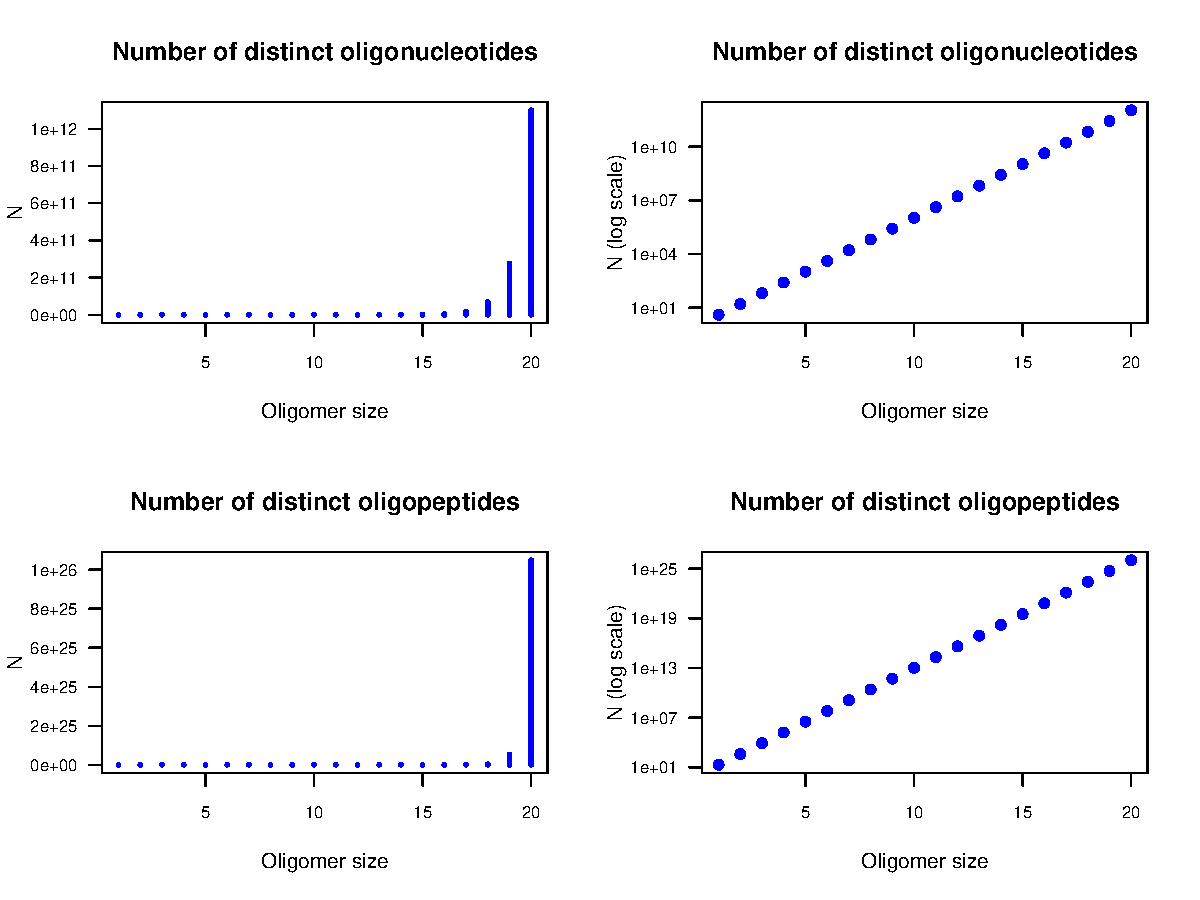
\includegraphics[width=0.6\linewidth]{figures/02_combinatorics_number_distinct_oligos-1} 

}

\caption{Number of possible oligonucleotides (top) and oligopeptides (bottom) with either a linear (left) and logarithmic (right) scale for the ordinate.}\label{fig:number_distinct_oligos}
\end{figure}

\end{frame}

\begin{frame}{Exercise 02.1: oligomers with no repeated residue}
\protect\hypertarget{exercise-02.1-oligomers-with-no-repeated-residue}{}

How many oligomers can be formed (DNA or peptides) that would contain
exactly once each residue.

\textbf{Suggested approach}: progressively aggregate the residues whilst
wondering, at each step, bow many residues have not yet been
incoroporated in the sequence.

\textbf{Sub-questions}:

\begin{itemize}
\item
  Generalise the formula for sequences of items of any type, drawn from
  a set of arbitrary size \(n\).
\item
  What is the name of the corresponding function?
\item
  In this process, what is the mode of residue selection: \textbf{with}
  or \textbf{without replacement}?
\end{itemize}

\end{frame}

\begin{frame}{Solution: oligomers with no repeated residue}
\protect\hypertarget{solution-oligomers-with-no-repeated-residue}{}

\begin{itemize}
\tightlist
\item
  First residue: \(n\) possibilities.
\item
  As soon as the first residue has been chosen, there are only \(n-1\)
  possibilities to draw a different residue for the second position. We
  thus have \(n \cdot (n-1)\) possible sequences for the first two
  residues.
\item
  For the third position, there are only \(n-2\) residues left; We thus
  have On a donc \(n \cdot (n-1) \cdot (n-2)\) possibilities for the 3
  first positions of the sequence.
\item
  By extension of this reasoning, the total number of possible solutions
  (assuming \(n\) is not too small) will be
\end{itemize}

\[n! = n \cdot (n-1) \cdot \ldots \cdot 2 \cdot 1\]

\begin{itemize}
\item
  In our case:

  \begin{itemize}
  \tightlist
  \item
    \(n! = 4! = 24\) oligonucléotides comportant exactement 1 fois
    chaque nucléotide (taille 4).
  \item
    \(n! = 20! = \ensuremath{2.43\times 10^{18}}\) oligopeptides (taille
    20).
  \end{itemize}
\end{itemize}

\end{frame}

\begin{frame}{The factorial function}
\protect\hypertarget{the-factorial-function}{}

\begin{itemize}
\tightlist
\item
  Enumerates the number of possible permutations of a finite set of
  items
\item
  Drawing withour replacement
\item
  Defined by a recursive formula
\end{itemize}

\[N = n! = \left\{
                \begin{array}{ll}
                  1 & \text{if } n=0 \\
                  n \cdot (n-1)! &\text{otherwise}
                \end{array}
              \right.\]

Note: by definition, \(0! = 1\), which enables to compute \(1!\) and the
subsequent numbers with the recursive formula.

For sufficiently large values of \(n\), a clearer formulation is

\[N = n \cdot (n-1) \cdot (n-2) \ldots 2 \cdot 1\]

\end{frame}

\begin{frame}{Factorial}
\protect\hypertarget{factorial}{}

\begin{center}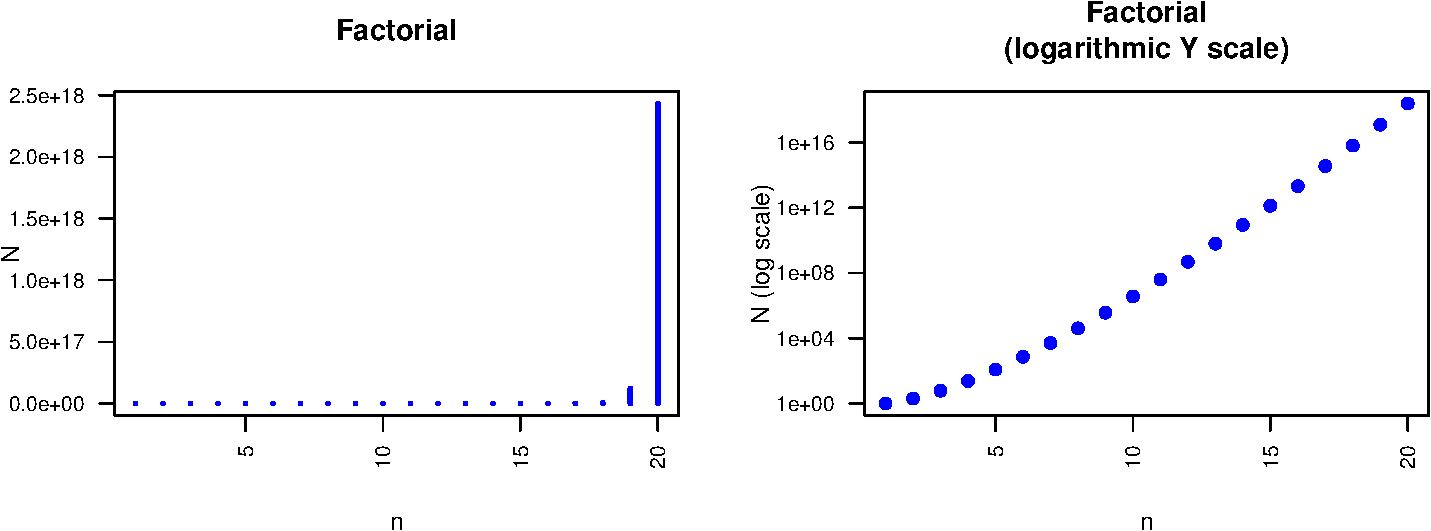
\includegraphics[width=0.95\linewidth]{figures/02_combinatorics_factorial-1} \end{center}

\end{frame}

\begin{frame}{Elements of combinatorics}
\protect\hypertarget{elements-of-combinatorics}{}

We summarize here the most widely used formulas in combinatorics.

\begin{itemize}
\tightlist
\item
  Arrangements (drawings with order, without replacement)
\item
  Combinations (drawings without considering the order of the items,
  without replacement)
\end{itemize}

\end{frame}

\begin{frame}{Arrangements}
\protect\hypertarget{arrangements}{}

In combinatorics, the term \textbf{arrangement} denotes an
\emph{orderless} drawing \emph{without replacement}, i.e.~random drawing
where the order of the item is taken in consideration, and where each
already selected item cannot be selected as next element.

Number of arrangements of \(x\) items drawn in a set of size \(n\).

\[\begin{array}{ccl}
A^x_n & = & \frac{n!}{(n - x)!} \\
 & = & \frac{n(n-1) \ldots (n-x +1) (n - x) (n-x-1) \ldots 2 \cdot 1}{(n - x) (n-x-1) \ldots 2 \cdot 1} \\
& = & n \cdot (n-1) \cdot \ldots \cdot (n-x+1)
\end{array}
\]

\end{frame}

\begin{frame}{Arrangements -- Typical application}
\protect\hypertarget{arrangements-typical-application}{}

\begin{itemize}
\item
  \href{https://en.wikipedia.org/wiki/Trifecta}{\textbf{tricast} (also
  named \textbf{trifecta}}).
\item
  A bet where players must predict the three winner horses (\(x=3\)) of
  a race, and the exact order of their arrival. For \(n=15\) horses,
  there are \(n \cdot (n-1) \cdot (n-2) = 15 \cdot 14 \cdot 13 = 2730\)
  possibilities.
\end{itemize}

\end{frame}

\begin{frame}{Exercise 02.2: gene lists (with order)}
\protect\hypertarget{exercise-02.2-gene-lists-with-order}{}

A transcriptome experiment has been led to define the level of
expression of all the yeast genes. Knowing that the genome contains
\(6000\) genes, how many possible ways are there to select the \(15\)
most expressed genes \emph{with their relative order}?

\textbf{Suggested approach}: as previously, simplify the problem by
starting from the minimal selection, and progressively increase the
number of selected genes (1 gène, 2 gènes, \ldots{}).

\textbf{Complementary questions}:

\begin{itemize}
\tightlist
\item
  Give the example of a familiar bet game related to this enumerating
  process.
\item
  Generalise the formula for any selection of a list of \(x\) items in a
  set containing \(n\) elements.
\end{itemize}

\end{frame}

\begin{frame}{Solution 02.2: listes (ordonnées) de gènes}
\protect\hypertarget{solution-02.2-listes-ordonnees-de-genes}{}

Il s'agit d'une sélection \textbf{sans remise} (chaque gène apparaît à
une et une seule position dans la liste de tous les gènes), et
\textbf{ordonnée} (les mêmes gènes pris dans un ordre différent sont
considérés comme un résultat différent).

\begin{itemize}
\tightlist
\item
  Pour le premier gène, il y a \(n=6000\) possibiité.
\item
  Dès le moment où on connaît le premier gène, il n'existe plus que 5999
  possibilités pour le second, et donc
  \(n \cdot (n-1) = 6000 \cdot 5999\) possibilités pour la suite des
  deux premiers gènes;
\item
  Par extension, il existe
  \(6000 \cdot 5999 \cdot 5998 \cdot \ldots \cdot 5986 = \ensuremath{4.62\times 10^{56}}\)
  possibilités pour les 15 premiers gènes.
\item
  En généralisant à la liste des \(x\) premiers gènes dans un ensemble
  de \(n\), on obtient
  \(N = n \cdot (n-1) \cdot (n-2) \cdot ... \cdot (n-x+1)\).
\end{itemize}

\end{frame}

\begin{frame}{Exercise 02.3: ensembles (non-ordonnés) de gènes}
\protect\hypertarget{exercise-02.3-ensembles-non-ordonnes-de-genes}{}

Lors d'une expérience de transcriptome indiquant le niveau d'expression
de tous les gènes de la levure. Sachant que le génome comporte 6000
gènes, combien de possibilité existe-t-il pour sélectionner les 15 gènes
les plus fortement exprimés (\textbf{sans tenir compte} de l'ordre
relatif de ces 15 gènes)?

\textbf{Approche suggérée}: comme précédemment, simplifiez le problème
en partant de sélections minimales (1 gène, 2 gènes, \ldots{}) et
généralisez la formule.

\textbf{Questions subsidiaires}:

\begin{itemize}
\tightlist
\item
  Trouvez un exemple familier de jeu de pari apparenté à ce problème.
\item
  Généralisez la formule pour la sélection d'un ensemble de \(x\) gènes
  dans un génome qui en comporte \(n\).
\item
  Connaissez-vous le nom de la formule ainsi trouvée?
\end{itemize}

\end{frame}

\begin{frame}{Solution 02.3: ensembles (non-ordonnés) de gènes}
\protect\hypertarget{solution-02.3-ensembles-non-ordonnes-de-genes}{}

\begin{itemize}
\tightlist
\item
  Pour une sélection d'un seul gène, il existe \(n=6000\) possibilité.
\item
  Pour 2 gènes, il existe \(n \cdot (n-1) = 6000 \cdot 5999\)
  arrangements, mais ceci inclut deux fois chaque paire de gènes
  (\((a, b)\) et \((b, a)\)). Le nombre d'ensembles non ordonnés est
  donc \(N = n \dot (n-1)/2\).
\item
  De même, pour 3 gènes, il faut diviser le nombre d'arrangements
  (\(A^x_n = \frac{n!}{(n-x)!} = 6000 \cdot 5999 \cdot 5998\)) par le
  nombre de permutations parmi tous les triplets de gènes
  (\((a, b, c), (a, c, b), (b, a, c) \ldots\)), ce qui donne
  \(\frac{6000!}{(6000-3)! 3!} = \frac{6000 \cdot 5999 \cdot 5888}{6} = \ensuremath{3.6\times 10^{10}}\).
\item
  Pour 15 gènes, on obtient
  \(\frac{n!}{(n-x)!x!} = \frac{6000!}{5985! \cdot 15!} = \ensuremath{3.53\times 10^{44}}\)
  \emph{combinations} possibles.
\end{itemize}

\end{frame}

\begin{frame}{Combinations}
\protect\hypertarget{combinations}{}

A \textbf{combination} is a selection \emph{without replacement} a
finite set, where the order of drawing is taken in considration.

The number of possible combinations of \(x\) numbers among \(n\) is
provided by the \textbf{bbinomial coefficient}.

\[\binom{n}{x} = C^x_n = \frac{n!}{x! (n-x)!}\]

\textbf{Attention: } the relative positions of \(x\) and \(n\) are
opposite in the two alternative notations for combinations
\(binom{n}{x}\) (``\(x\) among \(n\)'') and (\(C^x_n\), ``choose'').

\end{frame}

\begin{frame}{combinations -- Typical application}
\protect\hypertarget{combinations-typical-application}{}

\begin{itemize}
\tightlist
\item
  \href{https://en.wikipedia.org/wiki/Trifecta}{\textbf{trio}}, a
  variation of the \textbf{tricast} bet, where the order of arrival of
  the 3 winner horses is not taken in consideration.
\end{itemize}

\[\binom{n}{x} = \binom{15}{3} = C^3_{15} = \frac{15!}{3! 12!} = 455\]

\begin{itemize}
\tightlist
\item
  \href{https://fr.wikipedia.org/wiki/Loto}{\textbf{loto} (or lotto)}:
  each better checks 6 numbers within a grid containing 90 numbers. The
  number of possibilities is
\end{itemize}

\[\binom{n}{x} = \binom{90}{6} = C^6_{90} = \frac{90!}{6! 84!} = \ensuremath{6.2261463\times 10^{8}}\]

\end{frame}

\hypertarget{resume-des-concepts-et-formules}{%
\section{Résumé des concepts et
formules}\label{resume-des-concepts-et-formules}}

\begin{frame}{Tirages avec / sans remise}
\protect\hypertarget{tirages-avec-sans-remise}{}

Il existe deux types classiques de tirage d'éléments au sein d'un
ensemble: avec ou sans remise.

\begin{enumerate}
\item
  \textbf{Tirage sans remise}: chaque élément peut être tiré au plus une
  fois. Exemples:

  \begin{itemize}
  \tightlist
  \item
    Jeu de \href{https://fr.wikipedia.org/wiki/Loto}{loto} (ou lotto).
  \item
    Sélection aléatoire d'un ensemble de gènes dans un génome.
  \end{itemize}
\item
  Tirage \textbf{avec remise}: chaque élément peut être tiré zéro, une
  ou plusieurs fois. Exemples:

  \begin{itemize}
  \tightlist
  \item
    Jeu de dés. A chaque lancer on dispose des mêmes possibilités (6
    faces).
  \item
    Génération d'une séquence aléatoire, par sélection itérative d'un
    élément dans l'ensemble des résidus (4 nucléotides pour l'ADN, 20
    acides aminés pour les protéines).
  \end{itemize}
\end{enumerate}

\end{frame}

\begin{frame}{Choix de la formule}
\protect\hypertarget{choix-de-la-formule}{}

\begin{center}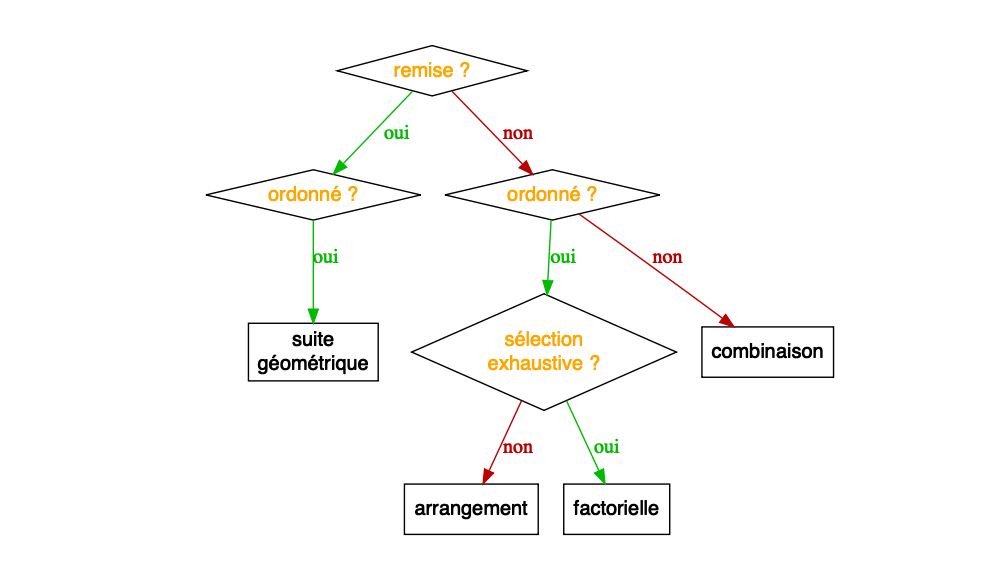
\includegraphics[width=0.9\linewidth]{figures/02_combinatorics_combinatorix_flowchart-1} \end{center}

\end{frame}

\begin{frame}{Formulas}
\protect\hypertarget{formulas}{}

\begin{longtable}[]{@{}llll@{}}
\toprule
\begin{minipage}[b]{0.12\columnwidth}\raggedright
Replacement\strut
\end{minipage} & \begin{minipage}[b]{0.10\columnwidth}\raggedright
Ordre\strut
\end{minipage} & \begin{minipage}[b]{0.18\columnwidth}\raggedright
Formula\strut
\end{minipage} & \begin{minipage}[b]{0.49\columnwidth}\raggedright
Description\strut
\end{minipage}\tabularnewline
\midrule
\endhead
\begin{minipage}[t]{0.12\columnwidth}\raggedright
Yes\strut
\end{minipage} & \begin{minipage}[t]{0.10\columnwidth}\raggedright
Yes\strut
\end{minipage} & \begin{minipage}[t]{0.18\columnwidth}\raggedright
\(n^x\)\strut
\end{minipage} & \begin{minipage}[t]{0.49\columnwidth}\raggedright
\textbf{Geometric progression}: ordered drawings (sequences), with
replacement, of \(x\) items from a set of size \(n\)\strut
\end{minipage}\tabularnewline
\begin{minipage}[t]{0.12\columnwidth}\raggedright
No\strut
\end{minipage} & \begin{minipage}[t]{0.10\columnwidth}\raggedright
Yes\strut
\end{minipage} & \begin{minipage}[t]{0.18\columnwidth}\raggedright
\(n!\)\strut
\end{minipage} & \begin{minipage}[t]{0.49\columnwidth}\raggedright
\textbf{factorial}: permutations of all elements of a set of size
\(n\)\strut
\end{minipage}\tabularnewline
\begin{minipage}[t]{0.12\columnwidth}\raggedright
No\strut
\end{minipage} & \begin{minipage}[t]{0.10\columnwidth}\raggedright
Yes\strut
\end{minipage} & \begin{minipage}[t]{0.18\columnwidth}\raggedright
\(A^x_n = \frac{n!}{(n-x)!}\)\strut
\end{minipage} & \begin{minipage}[t]{0.49\columnwidth}\raggedright
\textbf{Arrangements} : ordered drawing, without replacement, of \(x\)
items in a set of size \(n\)\strut
\end{minipage}\tabularnewline
\begin{minipage}[t]{0.12\columnwidth}\raggedright
No\strut
\end{minipage} & \begin{minipage}[t]{0.10\columnwidth}\raggedright
No\strut
\end{minipage} & \begin{minipage}[t]{0.18\columnwidth}\raggedright
\(C^x_n = \binom{n}{x} = \frac{n!}{x! (n - x) !}\)\strut
\end{minipage} & \begin{minipage}[t]{0.49\columnwidth}\raggedright
\textbf{Combinations} : orderless drawing, without replacement, of \(x\)
items in a set of size \(n\)\strut
\end{minipage}\tabularnewline
\bottomrule
\end{longtable}

\end{frame}

\hypertarget{supplementary-exercises}{%
\section{Supplementary exercises}\label{supplementary-exercises}}

\begin{frame}{Exercise~02.5: oligopeptides \(3 \times 20\)}
\protect\hypertarget{exercise02.5-oligopeptides-3-times-20}{}

\emph{How many distinct oligopeptides of size \(k=60\) can be formed by
using exactly \(3\) times each amino acid?}

\end{frame}

\begin{frame}[fragile]{Solution 02.5: oligopeptides \(3 \times 20\)}
\protect\hypertarget{solution-02.5-oligopeptides-3-times-20}{}

\emph{How many distinct oligopeptides of size \(k=60\) can be formed by
using exactly \(3\) times each amino acid?}

Commençons par générer une séquence particulière qui remplit ces
conditions, en concaténant 3 copies de chaque acide aminé, dans l'ordre
alphabétique.

\begin{verbatim}
AAACCCDDDEEEFFFGGGHHHIIIKKKLLLMMMNNNPPPQQQRRRSSSTTTVVVWWWYYY
\end{verbatim}

Toutes les permutations de ces 60 lettres sont des solutions valides. En
voici trois exemples.

\begin{verbatim}
<<<<<<< HEAD
VYCGYSPWCIKRKAFAPERNSTWERAPETQITNLLMNYIDQGFFCHDHSHWQGLVDKMMV
\end{verbatim}

\begin{verbatim}
RQLPMLEWGAGCRMKKNWNCAHNYERAYEFFMGKVWDIHLPPSSTDSFYHQQDIVTCVIT
\end{verbatim}

\begin{verbatim}
QYVINAHGEFEGFSPWMPNHYWSCEKDMTARYLTSKDQACGFIVQRKTPDRLILHNCMWV
=======
SIEYDPRTKCDDVFHAKPPGLNMMWIREFHEHCNMVVRSFCQIASLTYYWAWKGLGQTQN
\end{verbatim}

\begin{verbatim}
MEVPVSIRFHRCNSGIYDQAYMWYVCNATFFRSLNEACKHHWPQWPLKTLDTGKDGIMEQ
\end{verbatim}

\begin{verbatim}
TKKMWFSDTPHARYGRNFADCNENFYTYVEILKRCIQEPMPCGQDLHGHSVMIQWAWLSV
>>>>>>> 0084d050a30cebe47dfb962e8356abd3cd0eaa26
\end{verbatim}

Cependant, il faut prendre en compte le fait que certaines permutations
sont identiques (toutes celles où l'on permute deux acides aminés
identiques). La difficulté de l'Exercise sera donc de dénombrer le
nombre de permutations \emph{distinctes}.

\end{frame}

\end{document}
